\documentclass[11pt]{article}

\usepackage[margin=1in]{geometry}
\usepackage{amsmath,amssymb}
\usepackage{booktabs}
\usepackage{enumitem}
\usepackage{graphicx}
\usepackage[table]{xcolor}
\usepackage{microtype}
\usepackage[hidelinks]{hyperref}
\usepackage{url}
\usepackage{verbatim}

\newcommand{\placeholder}[1]{%
  \par\medskip
  \noindent\fcolorbox{black!45}{gray!8}{%
    \parbox{0.94\linewidth}{\textbf{Midpoint placeholder---not a result.} #1}}%
  \par\medskip
}
\newcommand{\miou}{\ensuremath{\mathrm{mIoU}}}
\newcommand{\iou}{\ensuremath{\mathrm{IoU}}}
\newcommand{\R}{\ensuremath{\mathbb{R}}}
\setlist{nosep,leftmargin=1.6em}
\frenchspacing

\title{\textbf{Terrain-Aware Semantic Segmentation for Autonomous Mars Rover Driving:}\\
CNNs vs. Transformers vs. Foundation Models\\[0.5em]
\large Midpoint Research Check-In}
\author{John Roth\\
EN.705.742---Advanced Applied Machine Learning, Summer 2026}
\date{July 2026}

\begin{document}
\maketitle

\begin{abstract}
Reliable terrain perception is a prerequisite for longer and safer autonomous Mars rover drives.
This project studies four-class semantic segmentation of rover navigation-camera imagery into
soil, bedrock, sand, and big rock using the public AI4Mars dataset. Although prior work established
that learned models can classify Martian terrain, a controlled and significance-tested comparison
of convolutional networks, vision transformers, and foundation-model references---including
transfer learning and cross-rover generalization---remains useful. The study compares U-Net and
DeepLabV3+ convolutional systems, SegFormer transformers, a small learned reference, a DINOv3 model
pretrained on Earth satellite imagery, and a Segment Anything mask-quality upper bound. All trained
systems use a common data protocol, loss, evaluation set, and reproducibility record. The primary
outcome is mean Intersection-over-Union, supplemented by per-class IoU and descriptive accuracy and
boundary measures. Hypotheses are evaluated with a preregistered paired seed/image bootstrap and
Holm correction, while cross-rover robustness is assessed by training on Curiosity and testing on
Opportunity/Spirit imagery. At this midpoint, 17 full-GPU runs provide descriptive evidence:
seven configurations have two completed seeds and three have one. Available-seed mean \miou{} is
approximately 0.80--0.82 for the conventional systems, compared with 0.681 for Tiny U-Net; a
single DINOv3-SAT seed reaches 0.840. Big-rock IoU remains substantially lower than the common
terrain classes. These values establish feasibility and motivate the remaining work, but
confirmatory H0--H5 decisions remain deferred until the complete three-seed experiment set is
available.
\end{abstract}

\section{Introduction}

Planetary rovers operate under communication delay, intermittent contact, limited bandwidth, and
strict safety constraints. A rover that can recognize the surface immediately ahead can select
safer paths and execute longer traverses without waiting for detailed ground commands. Pixel-level
terrain understanding is therefore an enabling perception capability: broad soil may be benign,
sand may create mobility risk, bedrock can produce wheel wear, and large rocks may be direct
hazards. The consequences are concrete. Curiosity accumulated wheel damage while traversing sharp
embedded rocks, motivating stronger onboard terrain assessment and systems such as Soil Property
and Object Classification (SPOC) \cite{rothrock2016spoc}.

AI4Mars makes a systematic machine-learning study of this task possible. Its merged public release
contains crowdsourced terrain annotations for rover imagery and smaller expert-agreement test sets
\cite{swan2021ai4mars,ai4marszenodo}. This project focuses on grayscale Curiosity navigation-camera
images because they are the stereo imagery used for driving and the release provides an expert test
split for that camera. A separate expert-labeled collection from the Mars Exploration Rovers
Opportunity and Spirit permits a stringent test of camera and terrain distribution shift.

The applied problem is dense multi-class semantic segmentation. Unlike image classification, the
model must preserve fine boundaries around rocks while also recognizing large, visually uniform
terrain regions. This tension motivates a comparison among three families of visual inductive bias.
U-Net and DeepLabV3+ use local convolution, skip connections, and multi-scale receptive fields
\cite{ronneberger2015unet,chen2018deeplab}. SegFormer uses hierarchical self-attention to capture
broader context \cite{xie2021segformer}. Foundation models bring priors learned from far larger
collections, although the difference between Earth imagery and ground-level Mars imagery makes
their transfer uncertain \cite{kirillov2023sam,simeoni2025dinov3}.

The central research question is:

\begin{quote}
For Mars terrain segmentation, how do convolutional, transformer, and foundation-model systems
compare; how much does pretrained initialization help; and how well does a Curiosity-trained system
generalize to Opportunity/Spirit imagery?
\end{quote}

The project makes four intended contributions. First, it provides a leakage-safe, reproducible
AI4Mars pipeline with explicit ignore-mask handling. Second, it compares representative CNN and
transformer systems under a shared training and evaluation protocol. Third, it measures transfer
learning and cross-rover generalization rather than reporting only a single in-domain score. Fourth,
it binds scientific claims to preregistered statistical decision rules. The last contribution is
especially important at the midpoint: successful prototype runs demonstrate feasibility, but they
are not treated as confirmatory evidence until all required seeds are complete.

\section{Related Work}

\subsection{Mars terrain perception}

SPOC demonstrated deep learning for terrain classification in Mars rover missions and connected
visual terrain labels to operational mobility needs \cite{rothrock2016spoc}. Swan et al. introduced
AI4Mars, combining rover images with crowdsourced labels and expert validation to support
terrain-aware autonomous driving research \cite{swan2021ai4mars}. The current merged-0.6 release is
distributed publicly through Zenodo \cite{ai4marszenodo}. More recent Mars-specific segmentation
work, including MarsSeg, explores specialized multi-level feature extraction
\cite{li2024marsseg}. These studies establish task relevance, but they do not resolve the controlled
combination of architecture family, initialization, cross-rover evaluation, and paired inference
addressed here.

\subsection{Convolutional semantic segmentation}

Fully convolutional networks replaced dense classification heads with spatial prediction and laid
the groundwork for end-to-end semantic segmentation \cite{long2015fcn}. U-Net combines a contracting
encoder with an expanding decoder and high-resolution skip connections, allowing semantic context
and localized boundary detail to interact \cite{ronneberger2015unet}. DeepLabV3+ instead emphasizes
multi-scale context through atrous spatial pyramid pooling and a decoder that refines object
boundaries \cite{chen2018deeplab}. Residual encoders provide deep, trainable feature hierarchies and
widely used ImageNet initialization \cite{he2016resnet,deng2009imagenet}. These CNNs supply strong
locality and translation priors that may be valuable when AI4Mars training data is limited or
labels are noisy.

\subsection{Transformers and foundation models}

The Vision Transformer showed that attention-based models can learn visual representations from
sequences of image patches \cite{dosovitskiy2021vit}. SegFormer adapts hierarchical transformer
features to semantic segmentation with efficient sequence reduction and a lightweight decoder
\cite{xie2021segformer}. Its global context may help with broad soil and sand regions, although its
boundary behavior and data requirements must be measured rather than assumed.

Segment Anything (SAM) was trained on more than a billion masks and produces class-agnostic regions
from prompts \cite{kirillov2023sam}. AI4Mars provides no semantic prompt channel, so SAM is not
treated here as deployable zero-shot terrain classification. Instead, a preregistered region-oracle
assignment measures an explicit upper bound on what a semantic labeler could obtain from SAM's mask
proposals. DINOv3 is a 2025 Meta AI research preprint on self-supervised visual representation
learning at scale \cite{simeoni2025dinov3}; it is not described as peer reviewed. Its SAT-493M
variant is nevertheless scientifically interesting because it transfers features learned from
Earth orbital imagery to ground-level Mars imagery. That cross-planet and cross-viewpoint gap makes
the reference a test of representation transfer, not an assumed advantage.

\section{Research Project Problem}

\subsection{Task definition and scope}

Let a grayscale navigation-camera image be
$\mathbf{x}\in\R^{H\times W}$. It is replicated across three channels for compatibility with
pretrained encoders. A segmentation model
$f_{\theta}:\R^{H\times W\times 3}\rightarrow\R^{H\times W\times C}$ produces logits for
$C=4$ terrain classes. The predicted label map is
\begin{equation}
\hat{y}_{ij}=\arg\max_{c\in\{0,1,2,3\}} f_{\theta}(\mathbf{x})_{ijc},
\end{equation}
where the classes are soil, bedrock, sand, and big rock. Ground-truth value 255 denotes ignored
pixels, including unlabeled regions, rover hardware, or regions outside the labeling range. Ignored
pixels contribute to neither training loss nor evaluation metrics.

The primary in-rover dataset contains 16,064 labeled Curiosity Navcam training images and 322
expert-labeled test images from the pinned
\path{masked-gold-min3-100agree} subset. The training images are split by image into 12,851 training
and 3,213 validation records using seed 1414. Curiosity Mastcam imagery is out of scope because it
is a different color science camera without the corresponding gold test protocol. The cross-rover
test contains 204 expert-labeled Opportunity/Spirit images and is never used for training.

\subsection{Research gap}

Individual Mars segmentation systems can achieve useful performance, but a reported score alone
does not identify why it is high or whether it will transfer. Architecture, pretrained
initialization, class imbalance, seed variation, and rover/camera domain shift may all influence an
observed result. The project addresses this gap with controlled within-architecture initialization
comparisons, configured cross-family comparisons, per-class analysis, and paired uncertainty
estimation over both training seed and test image.

\subsection{Hypotheses}

The executable hypothesis definitions are frozen in \path{configs/hypotheses.yaml}; the summary
below follows the current protocol rather than superseded proposal wording.

\begin{description}[leftmargin=3em,style=nextline]
  \item[H0] No tested deep system significantly exceeds the constant-majority reference on
  \miou. H0 is rejected exactly when H1 is supported; otherwise the study reports failure to reject,
  not evidence that the systems are equivalent.
  \item[H1] At least one conventional deep system---U-Net, DeepLabV3+, or SegFormer---exceeds the
  constant-majority reference on \miou under the Family-A adjusted test.
  \item[H2] Pretrained initialization improves at least one tested architecture relative to its
  backbone-matched from-scratch counterpart. The inference is deliberately bounded and does not
  claim that pretraining helps every architecture.
  \item[H3] Configured SegFormer MiT-B2 systems differ from the configured U-Net with ResNet-34 or
  DeepLabV3+ with ResNet-50 systems overall or for at least one terrain class. Effects are reported as
  configured-system differences, not as a pure causal effect of attention.
  \item[H4] The validation-selected conventional system has a Curiosity-to-MER \miou{} drop below
  0.15 and a cross-rover 90\% confidence-interval lower bound above the MER majority reference.
  \item[H5] DINOv3-SAT or the SAM region-oracle upper bound exceeds the learned Tiny U-Net reference
  under the gated Family-E comparison. Missing gated weights or incomplete learned seed sets defer
  this hypothesis.
\end{description}

\section{Method}

\subsection{Data pipeline and leakage controls}

The dataset index pairs image and label paths within a single rover/camera subtree and assigns each
image a stable, camera-qualified name. Splits operate on those image records rather than on crops,
so a frame cannot occur in both training and validation sets. The official expert test images are
held out from model and hyperparameter selection. The MER set is test-only. Preflight checks assert
the expected record counts, image/label pairing, split disjointness, permitted mask values, and
archive/index fingerprints.

Images are decoded as grayscale and replicated to three channels. Training and evaluation resize
to $512\times512$ pixels and use ImageNet normalization. The frozen augmentation recipe allows a
horizontal flip and mild brightness/contrast perturbation. It excludes vertical flips because
inverting the horizon is physically implausible. Nearest-neighbor mask interpolation preserves
categorical labels. Class weights are computed from training-split pixel frequencies and clipped to
avoid unstable extremes.

\subsection{Compared systems}

\begin{table}[ht]
\centering
\caption{Planned systems and their roles in the preregistered study.}
\small
\begin{tabular}{@{}llll@{}}
\toprule
System & Backbone/variant & Initialization & Protocol role \\
\midrule
Majority & Constant soil & None & H1/H4 non-learned reference \\
Tiny U-Net & Two-level CNN & Random & H5 learned reference \\
U-Net & ResNet-34 & ImageNet / random & CNN and H2 comparison \\
DeepLabV3+ & ResNet-50 & ImageNet / random & Multi-scale CNN and H2 \\
SegFormer & MiT-B0/B2 & ImageNet / random & Transformer and H2/H3 \\
DINOv3-SAT & ViT-L/16 SAT-493M & Self-supervised & Gated H5 reference \\
SAM & ViT-B proposals & Foundation weights & Region-oracle upper bound \\
\bottomrule
\end{tabular}
\end{table}

The Tiny U-Net contains two encoder/decoder levels and is intentionally small. U-Net fuses encoder
and decoder features through skip connections. For encoder feature $\mathbf{e}_{\ell}$ and deeper
decoder feature $\mathbf{d}_{\ell+1}$, a decoder stage has the schematic form
\begin{equation}
\mathbf{d}_{\ell}=\operatorname{Conv}\left(
[\operatorname{Up}(\mathbf{d}_{\ell+1});\mathbf{e}_{\ell}]\right).
\end{equation}
DeepLabV3+ uses atrous convolution to enlarge the receptive field without reducing feature-map
resolution. For dilation $r$,
\begin{equation}
y[i]=\sum_k x[i+r k]w[k].
\end{equation}
SegFormer uses hierarchical Mix-Transformer features. Its attention operation is
\begin{equation}
\operatorname{Attention}(Q,K,V)=
\operatorname{softmax}\left(\frac{QK^{\mathsf T}}{\sqrt{d}}\right)V,
\end{equation}
with sequence reduction to control cost at image resolution.

The DINOv3-SAT arm uses a satellite-pretrained visual backbone with a trained segmentation head.
The SAM arm generates class-agnostic proposals. For its oracle upper bound, each proposal receives
the majority ground-truth class among its valid pixels; later proposals overwrite earlier ones and
uncovered pixels default to soil. Because this procedure consults the target label, it is explicitly
an analysis upper bound and cannot be represented as deployable inference.

\subsection{Optimization objective}

All trained conventional systems minimize class-weighted cross-entropy plus soft Dice loss over
valid pixels:
\begin{equation}
\mathcal{L}=\mathcal{L}_{\mathrm{CE}}^{w}(\hat{\mathbf y},\mathbf y)
+\lambda\left(1-\operatorname{Dice}(\hat{\mathbf y},\mathbf y)\right),
\end{equation}
\begin{equation}
\operatorname{Dice}=\frac{2\sum p g+\epsilon}{\sum p+\sum g+\epsilon}.
\end{equation}
The validity mask is applied to both terms. Optimization uses AdamW
\cite{loshchilov2019adamw}; validation \miou{} controls model selection, and the expert test set is
not used to choose an epoch or configuration.

\subsection{Evaluation measures}

For class $c$, Intersection-over-Union is
\begin{equation}
\operatorname{IoU}_{c}=\frac{\mathrm{TP}_{c}}
{\mathrm{TP}_{c}+\mathrm{FP}_{c}+\mathrm{FN}_{c}}.
\end{equation}
The primary metric, \miou, is the macro mean over the fixed set of classes present in the full
evaluation split. Per-class IoU is essential because the common soil class can obscure failures on
the drivability-relevant big-rock class. Pixel accuracy and boundary-F1 at three-pixel tolerance are
reported descriptively but are not hypothesis-tested. Per-image integer intersections, unions,
correct pixels, and valid-pixel counts are stored so aggregate metrics can be reconstructed under
resampling without retaining predicted masks.

\subsection{Statistical protocol}

Learned confirmatory arms require training seeds 1414, 1415, and 1416. Deterministic references are
computed once and paired against each learned seed. The primary inference uses 10,000 paired
bootstrap resamples, first over training seeds and then over images within a seed, with purpose seed
0 reset per comparison. The study reports percentile 90\% confidence intervals and plus-one
p-values. Family A and B tests are one-sided in their preregistered positive directions; Family C is
two-sided and includes overall and fixed-set per-class comparisons in one correction family.
Holm's procedure controls multiplicity within each hypothesis family at $\alpha=0.10$
\cite{holm1979simple}. H4 uses its preregistered threshold-plus-interval rule rather than a p-value.

Every run records its resolved configuration, seed, git revision, configuration/code hash, package
versions, hardware profile, parameter counts, timestamps, and per-image sufficient statistics.
This manifest-based design separates reproducibility evidence from large untracked checkpoints and
raw data.

\subsection{End-to-end pipeline}

\begin{verbatim}
AI4Mars MSL Navcam images + labels (255 = ignore)
              |
camera-scoped index -> by-image train/validation split
              |
resize, safe augmentation, normalization, class weights
              |
 +------------+-------------+------------+----------------+
 | U-Net      | DeepLabV3+  | SegFormer  | DINOv3 / SAM  |
 +------------+-------------+------------+----------------+
              |
weighted cross-entropy + Dice (valid pixels only)
              |
MSL expert test + MER cross-rover test
              |
per-image counts -> paired seed/image bootstrap -> Holm
\end{verbatim}

\section{Experimental Progress and Collection Plan}

The implementation and bounded notebook prototype establish that images, labels, transforms,
models, loss, and metrics can be connected. The current result store contains 17 successful
full-GPU in-rover \miou{} records spanning ten configurations. Seven configurations have completed
seeds 1414 and 1415; SegFormer B2 pretrained, SegFormer B2 scratch, and DINOv3-SAT currently have
seed 1414 only. Table~\ref{tab:inventory} makes the remaining work explicit. An \emph{complete}
entry means that a test artifact and per-image sufficient statistics exist, not that the comparison
is confirmatory.

\begin{table}[ht]
\centering
\caption{Midpoint full-GPU run inventory. Both initialization variants have the same status where
shown as a pair. Seed 1416 is required before confirmatory inference.}
\label{tab:inventory}
\begin{tabular}{@{}lllll@{}}
\toprule
System & Variant & 1414 & 1415 & 1416 \\
\midrule
Tiny U-Net & scratch & complete & complete & pending \\
U-Net R34 & pretrained / scratch & complete & complete & pending \\
DeepLabV3+ R50 & pretrained / scratch & complete & complete & pending \\
SegFormer B0 & pretrained / scratch & complete & complete & pending \\
SegFormer B2 & pretrained / scratch & complete & pending & pending \\
DINOv3-SAT & finetuned & complete & pending & pending \\
SAM oracle & deterministic & pending & --- & --- \\
\bottomrule
\end{tabular}
\end{table}

\begin{figure}[ht]
\centering
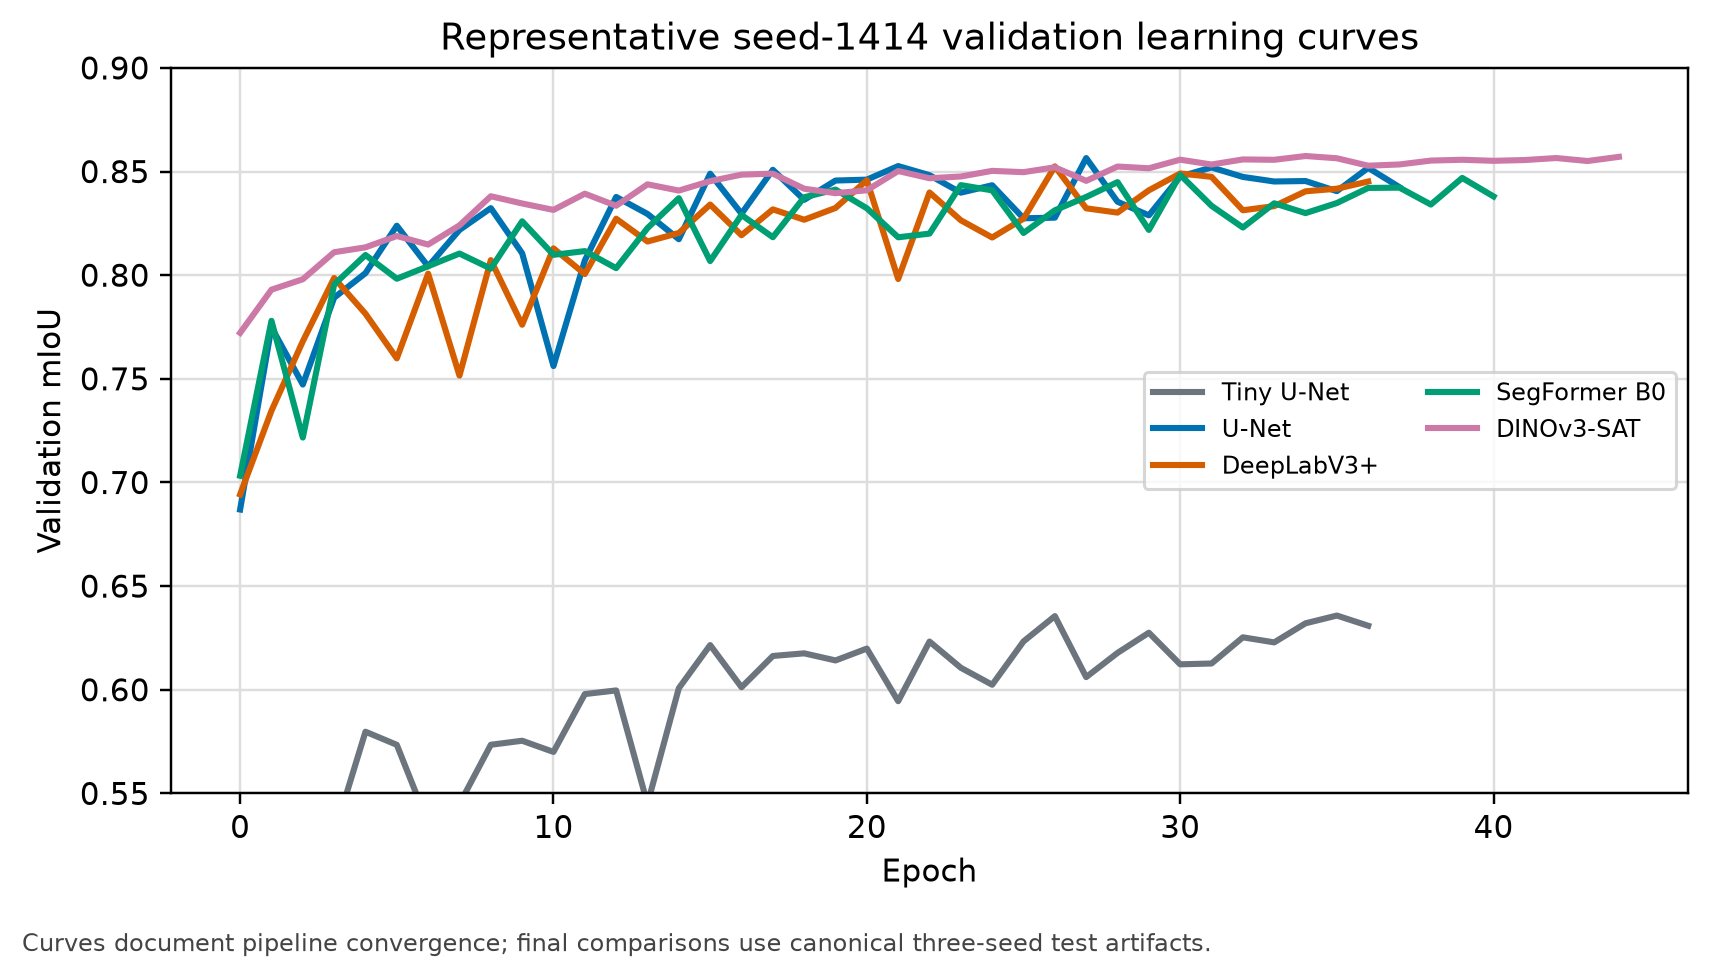
\includegraphics[width=0.92\linewidth]{figures/training_curves.png}
\caption{Representative seed-1414 validation learning curves. These curves demonstrate stable
optimization and model-selection feasibility; they are not hypothesis tests.}
\label{fig:curves}
\end{figure}

\begin{figure}[ht]
\centering
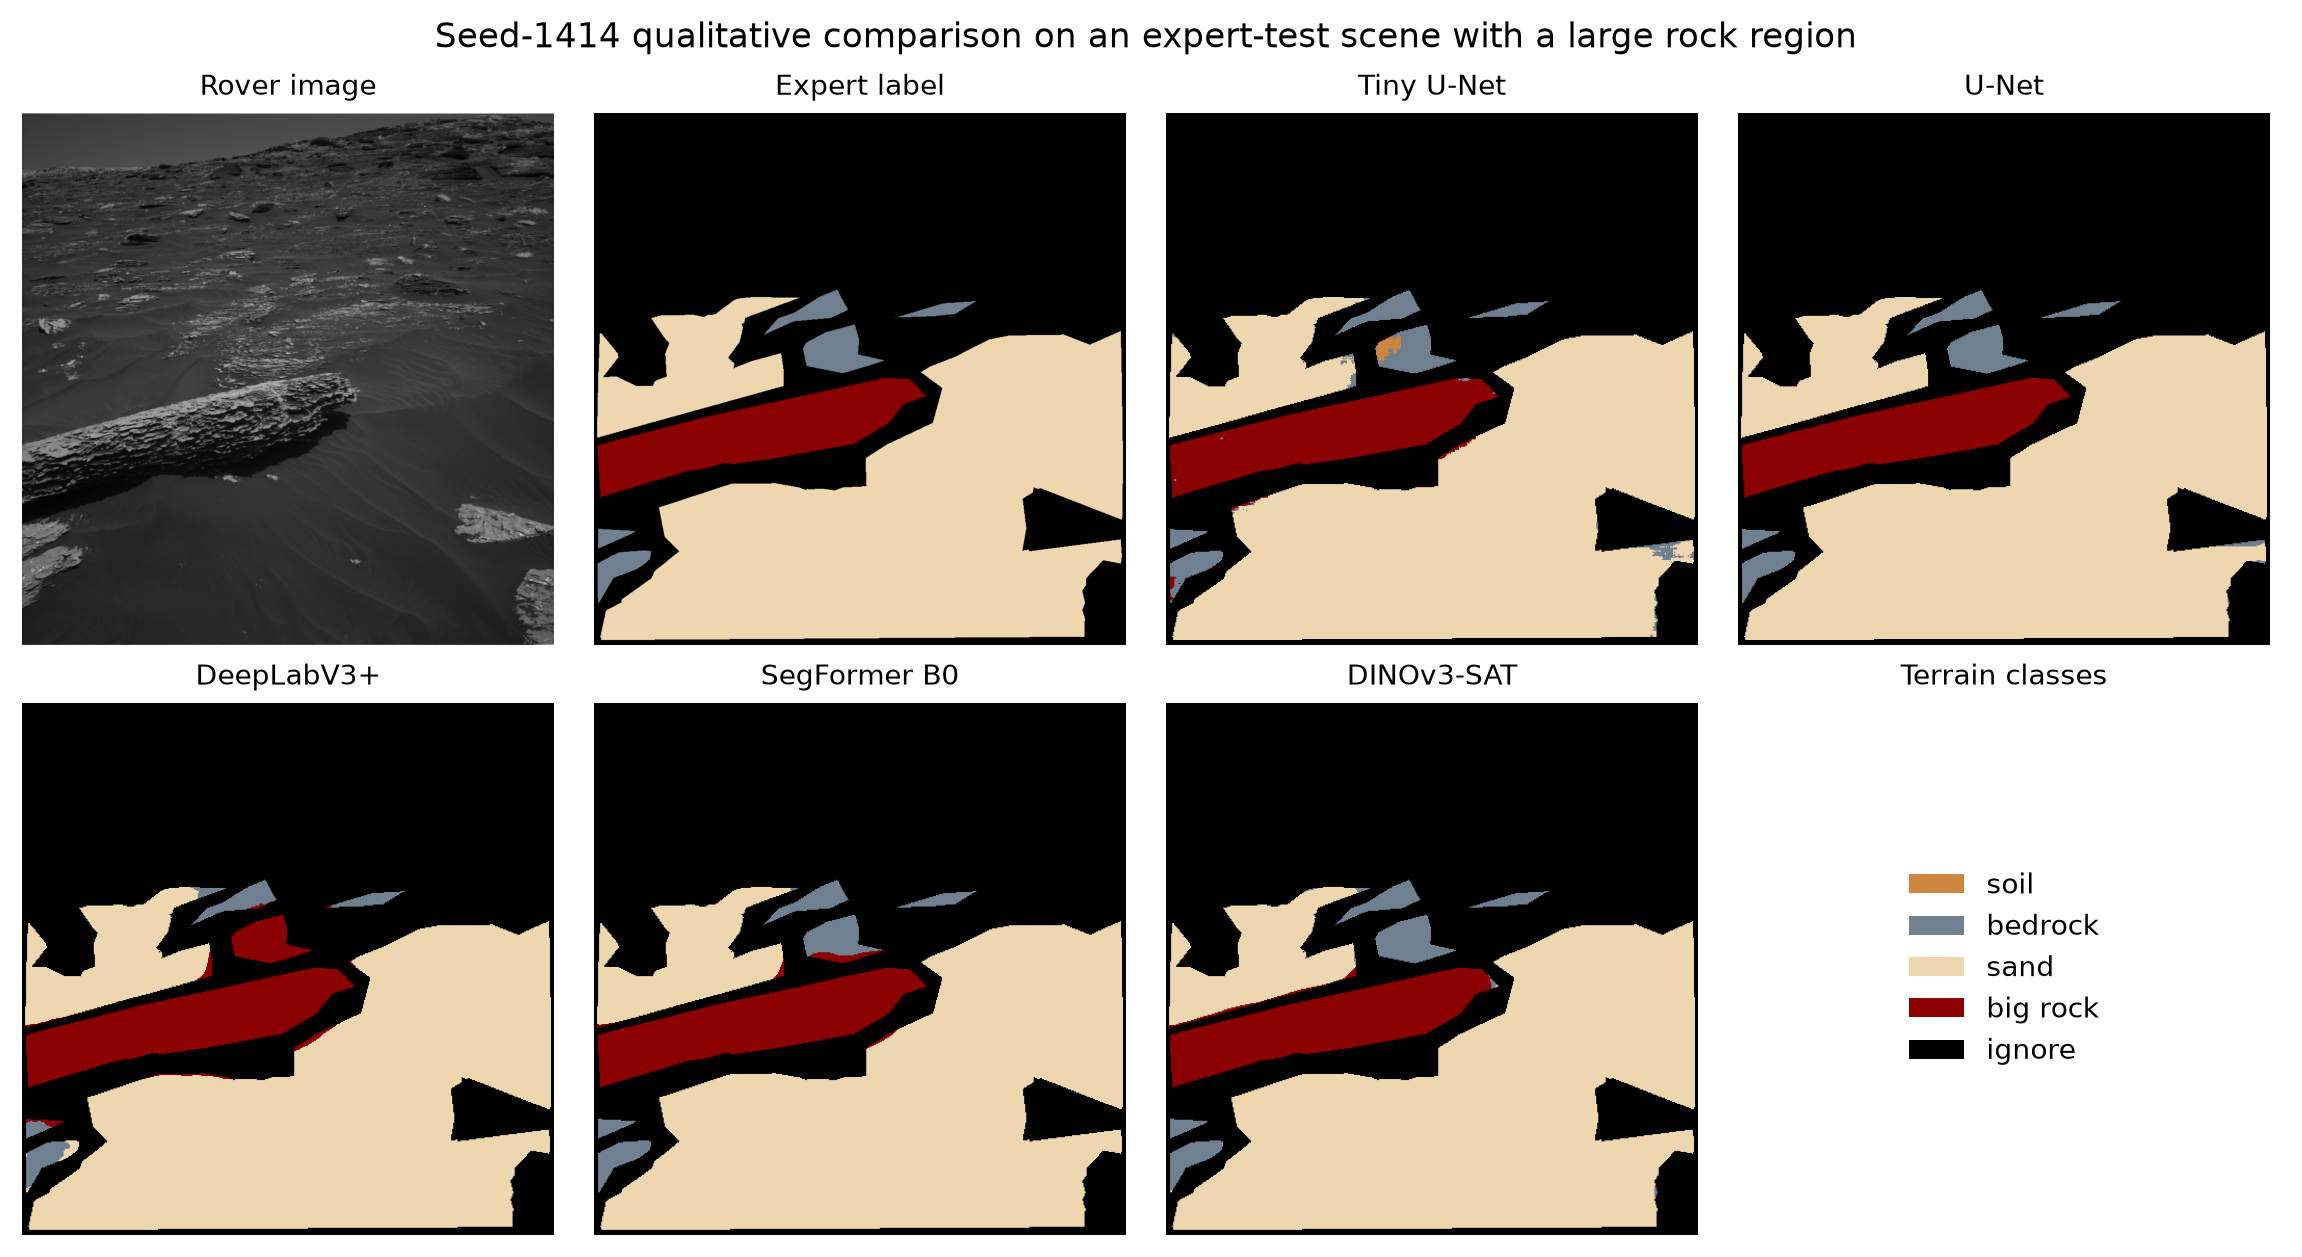
\includegraphics[width=\linewidth]{figures/qualitative_predictions.png}
\caption{A fixed expert-test scene containing a large rock region, shown with the expert label and
seed-1414 predictions. Black pixels are ignored. The example was selected for rare-class coverage,
not because it maximized any model's score.}
\label{fig:qualitative}
\end{figure}

\section{Statistical Analysis and Results}

\subsection{Preliminary descriptive results}

Table~\ref{tab:overall} reports the evidence currently available. For two-seed configurations,
\miou{} is the arithmetic mean with the sample standard deviation across seeds in parentheses.
Per-class values are available-seed means. DINOv3-SAT has only one completed seed, so neither a
seed standard deviation nor a fair stability comparison is yet possible. These are descriptive
summaries; the preregistered hierarchical bootstrap is not approximated with a two-seed test.

\begin{table}[ht]
\centering
\caption{Preliminary in-rover expert-test performance. SD is across available training seeds;
the DINOv3-SAT entry is a single run.}
\label{tab:overall}
\small
\begin{tabular}{@{}lrrrrrr@{}}
\toprule
System & $n$ & \miou{} mean (SD) & Soil & Bedrock & Sand & Big rock \\
\midrule
Tiny U-Net scratch & 2 & 0.681 (0.002) & 0.918 & 0.837 & 0.873 & 0.094 \\
U-Net R34 pretrained & 2 & 0.821 (0.018) & 0.979 & 0.942 & 0.962 & 0.399 \\
U-Net R34 scratch & 2 & 0.822 (0.001) & 0.983 & 0.933 & 0.962 & 0.409 \\
DeepLabV3+ R50 pretrained & 2 & 0.817 (0.022) & 0.982 & 0.937 & 0.966 & 0.382 \\
DeepLabV3+ R50 scratch & 2 & 0.819 (0.012) & 0.980 & 0.940 & 0.967 & 0.388 \\
SegFormer B0 pretrained & 2 & 0.816 (0.016) & 0.981 & 0.940 & 0.964 & 0.379 \\
SegFormer B0 scratch & 2 & 0.802 (0.004) & 0.960 & 0.897 & 0.908 & 0.444 \\
DINOv3-SAT finetuned & 1 & 0.840 (---) & 0.981 & 0.940 & 0.970 & 0.469 \\
\bottomrule
\end{tabular}
\end{table}

\begin{figure}[ht]
\centering
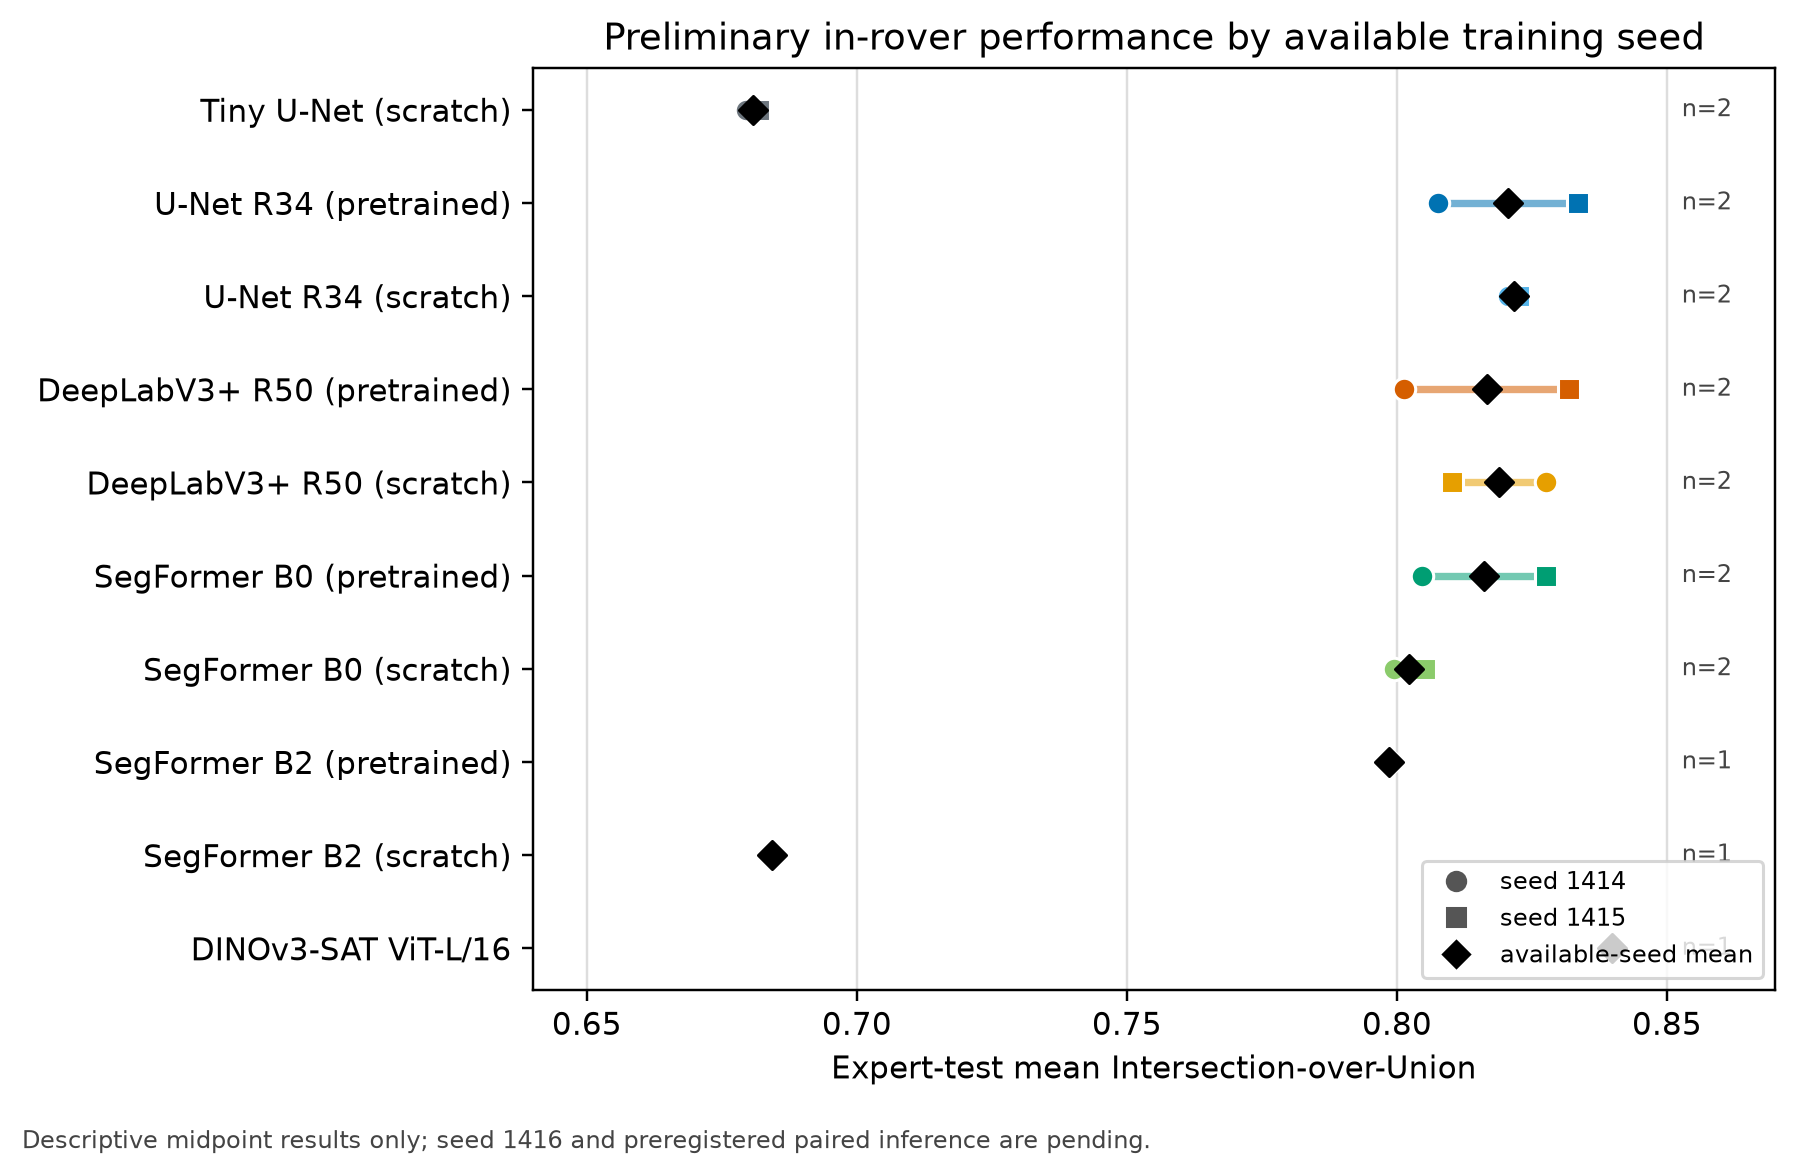
\includegraphics[width=0.94\linewidth]{figures/preliminary_miou.png}
\caption{Every available full-GPU in-rover \miou{} result. Points show individual seeds; black
diamonds show the mean of the currently available seeds. Connecting lines are descriptive ranges,
not confidence intervals.}
\label{fig:prelim-miou}
\end{figure}

Across the two-seed conventional configurations, mean \miou{} lies in a narrow band from 0.802 to
0.822. U-Net scratch has the largest available-seed mean (0.822), but it differs from pretrained
U-Net by only 0.001 and seed 1414 and 1415 favor different variants. DeepLabV3+ shows the same
directionally inconsistent pattern. SegFormer B0 is the only two-seed architecture for which the
available mean favors pretraining (0.816 versus 0.802). These mixed directions are exactly why H2
must remain unresolved until seed 1416 and the paired test are complete.

The single DINOv3-SAT run has the highest observed point estimate, 0.840, and the highest currently
observed big-rock IoU among the representative systems, 0.469. This is promising evidence for
continuing H5, not evidence that H5 is supported. Across every representative system, soil,
bedrock, and sand IoUs are high, while big-rock IoU is substantially lower. The class-level pattern
suggests that rare hazard segmentation, rather than broad terrain labeling, is the principal
remaining error mode. Figure~\ref{fig:qualitative} illustrates both strong broad-region agreement
and visibly different handling of the large-rock boundary.

\placeholder{Populate the cross-rover table with the validation-selected conventional system,
its MSL and MER \miou, their difference, the MER hierarchical confidence interval, and the MER
majority score. Apply the exact H4 threshold rule without substituting a post hoc test.}

\subsection{Confirmatory analysis still pending}

\begin{table}[ht]
\centering
\caption{Preregistered hypothesis tests (confirmatory placeholder).}
\label{tab:tests}
\begin{tabular}{@{}llllll@{}}
\toprule
Hypothesis & Comparison & Effect & 90\% CI & Holm $p$ & Decision \\
\midrule
H1 & deep vs. majority & TBD & TBD & TBD & deferred \\
H2 & pretrained vs. scratch & TBD & TBD & TBD & deferred \\
H3 & SegFormer vs. CNNs & TBD & TBD & TBD & deferred \\
H4 & MSL-to-MER drop & TBD & TBD & n/a & deferred \\
H5 & foundation vs. Tiny U-Net & TBD & TBD & TBD & deferred \\
\bottomrule
\end{tabular}
\end{table}

At the midpoint, every hypothesis remains deferred. The descriptive results above document progress
without converting partial seed sets into adjusted p-values or hypothesis decisions. Final
inference will be generated only after canonical selection verifies the required run set and the
executable protocol snapshot matches the preregistration.

\section{Discussion and Limitations}

\placeholder{Interpret only supported, multiplicity-corrected effects. Discuss whether observed
differences are practically meaningful for terrain classes, not merely statistically detectable.
Relate overall results to parameter counts and per-class/boundary behavior without turning the
configured-system comparisons into architecture-only causal claims.}

The preliminary evidence already identifies useful questions for the final discussion. First,
conventional architecture point estimates are much closer to one another than they are to Tiny
U-Net, so uncertainty and paired effects will matter more than rank ordering. Second, the available
pretraining effects are small and inconsistent across seeds for the CNNs. Third, the highest
single-seed point belongs to DINOv3-SAT, but its stability is unknown. Finally, all systems show a
large gap between common terrain and big rock. This gap has direct operational relevance because a
rare large rock can matter more to a rover path than another correctly labeled patch of soil.

Several limitations are known before results. AI4Mars labels combine crowdsourced judgments and
expert-agreement subsets, so both class ambiguity and annotation noise matter. The primary scope is
grayscale Navcam imagery and does not establish performance on Mastcam, orbital imagery, or future
rovers. MER tests domain shift but cannot identify whether any degradation arises from camera,
mission, lighting, geography, or all four. Big rock is rare, making its estimate more variable than
common-class estimates. Three training seeds improve uncertainty accounting but do not exhaust the
space of optimization outcomes. Finally, SAM's region-oracle assignment uses target labels and is
only an upper bound; it cannot be presented as an autonomous semantic-segmentation system.

\section{Conclusion}

\placeholder{State the final answer to the research question after H0--H5 are evaluated. Summarize
which configured system performs best, whether transfer helps any architecture, which classes show
material differences, and whether cross-rover degradation meets the preregistered bound. Connect
the evidence to rover drivability and identify the next most defensible experiment.}

This midpoint establishes the research problem, literature position, controlled method, runnable
prototype, descriptive results from 17 full-GPU runs, and statistical collection plan. The current
evidence shows that the pipeline learns strong broad-terrain segmentations and that rare big-rock
recognition remains difficult. It intentionally does not convert incomplete experiment runs into
confirmatory scientific conclusions.

\section*{Data and Code Availability}

The AI4Mars merged-0.6 archive is publicly available from Zenodo record 15995036
\cite{ai4marszenodo}. The expected archive is approximately 16.2 GB with MD5
\texttt{daf80a86021253292e6c425f97baa5c6}. It is not included with this submission. The accompanying
notebook provides download, integrity-check, and expected-layout instructions and uses the project
code directly. Raw data, model weights, secrets, checkpoints, and generated prediction masks remain
excluded from version control.

\begin{thebibliography}{99}

\bibitem{swan2021ai4mars}
R. M. Swan, D. Atha, H. A. Leopold, et al., ``AI4MARS: A Dataset for Terrain-Aware Autonomous
Driving on Mars,'' in \emph{Proceedings of the IEEE/CVF Conference on Computer Vision and Pattern
Recognition Workshops}, 2021.

\bibitem{ai4marszenodo}
NASA Jet Propulsion Laboratory, ``AI4Mars: A Dataset for Terrain-Aware Autonomous Driving on Mars,
merged-0.6,'' Zenodo, record 15995036, 2025. Available:
\url{https://zenodo.org/records/15995036}.

\bibitem{rothrock2016spoc}
B. Rothrock, R. Kennedy, C. Cunningham, J. Papon, M. Heverly, and M. Ono, ``SPOC: Deep
Learning-Based Terrain Classification for Mars Rover Missions,'' in \emph{AIAA SPACE 2016}, 2016.

\bibitem{li2024marsseg}
Y. Li et al., ``MarsSeg: Mars Surface Semantic Segmentation with Multi-level Extractor and
Connector,'' arXiv:2404.04155, 2024. Research preprint.

\bibitem{long2015fcn}
J. Long, E. Shelhamer, and T. Darrell, ``Fully Convolutional Networks for Semantic Segmentation,''
in \emph{Proceedings of CVPR}, 2015.

\bibitem{ronneberger2015unet}
O. Ronneberger, P. Fischer, and T. Brox, ``U-Net: Convolutional Networks for Biomedical Image
Segmentation,'' in \emph{Proceedings of MICCAI}, 2015.

\bibitem{chen2018deeplab}
L.-C. Chen, Y. Zhu, G. Papandreou, F. Schroff, and H. Adam, ``Encoder-Decoder with Atrous Separable
Convolution for Semantic Image Segmentation,'' in \emph{Proceedings of ECCV}, 2018.

\bibitem{xie2021segformer}
E. Xie, W. Wang, Z. Yu, A. Anandkumar, J. M. Alvarez, and P. Luo, ``SegFormer: Simple and Efficient
Design for Semantic Segmentation with Transformers,'' in \emph{Advances in Neural Information
Processing Systems}, vol. 34, 2021.

\bibitem{kirillov2023sam}
A. Kirillov, E. Mintun, N. Ravi, et al., ``Segment Anything,'' in \emph{Proceedings of ICCV}, 2023.

\bibitem{simeoni2025dinov3}
O. Sim\'eoni et al., ``DINOv3: Self-Supervised Learning for Vision at Scale,'' arXiv:2508.10104,
2025. Meta AI research preprint.

\bibitem{he2016resnet}
K. He, X. Zhang, S. Ren, and J. Sun, ``Deep Residual Learning for Image Recognition,'' in
\emph{Proceedings of CVPR}, 2016.

\bibitem{dosovitskiy2021vit}
A. Dosovitskiy et al., ``An Image Is Worth 16$\times$16 Words: Transformers for Image Recognition
at Scale,'' in \emph{Proceedings of ICLR}, 2021.

\bibitem{deng2009imagenet}
J. Deng, W. Dong, R. Socher, L.-J. Li, K. Li, and L. Fei-Fei, ``ImageNet: A Large-Scale Hierarchical
Image Database,'' in \emph{Proceedings of CVPR}, 2009.

\bibitem{milletari2016vnet}
F. Milletari, N. Navab, and S.-A. Ahmadi, ``V-Net: Fully Convolutional Neural Networks for
Volumetric Medical Image Segmentation,'' in \emph{Proceedings of 3DV}, 2016.

\bibitem{loshchilov2019adamw}
I. Loshchilov and F. Hutter, ``Decoupled Weight Decay Regularization,'' in \emph{Proceedings of
ICLR}, 2019.

\bibitem{efron1993bootstrap}
B. Efron and R. J. Tibshirani, \emph{An Introduction to the Bootstrap}. Chapman \& Hall, 1993.

\bibitem{holm1979simple}
S. Holm, ``A Simple Sequentially Rejective Multiple Test Procedure,'' \emph{Scandinavian Journal
of Statistics}, vol. 6, no. 2, pp. 65--70, 1979.

\bibitem{everingham2010voc}
M. Everingham, L. Van Gool, C. K. I. Williams, J. Winn, and A. Zisserman, ``The PASCAL Visual
Object Classes Challenge,'' \emph{International Journal of Computer Vision}, vol. 88, pp. 303--338,
2010.

\end{thebibliography}

\end{document}
